\chapter{Results}\label{ch:Results}

\section{Linear Modelling}

\subsection{Length of Comment vs Comment Score}
    The first potential linear relation that was examined was to see if the length of the comment could be used as a predictor of the score of the comment. The length of the comment was measured based on the number of characters within the \textit{body} field of the comment. Firstly a simple graph was plotted of the score of each comment vs the length of the comment, this can be seen in \autoref{fig:scorevlen} below. This proved to be extremely unhelpful due to the fact that there are so many comments with a score of 0, which is unclear in the plot.
    
    \begin{figure}[H]
        \centering
        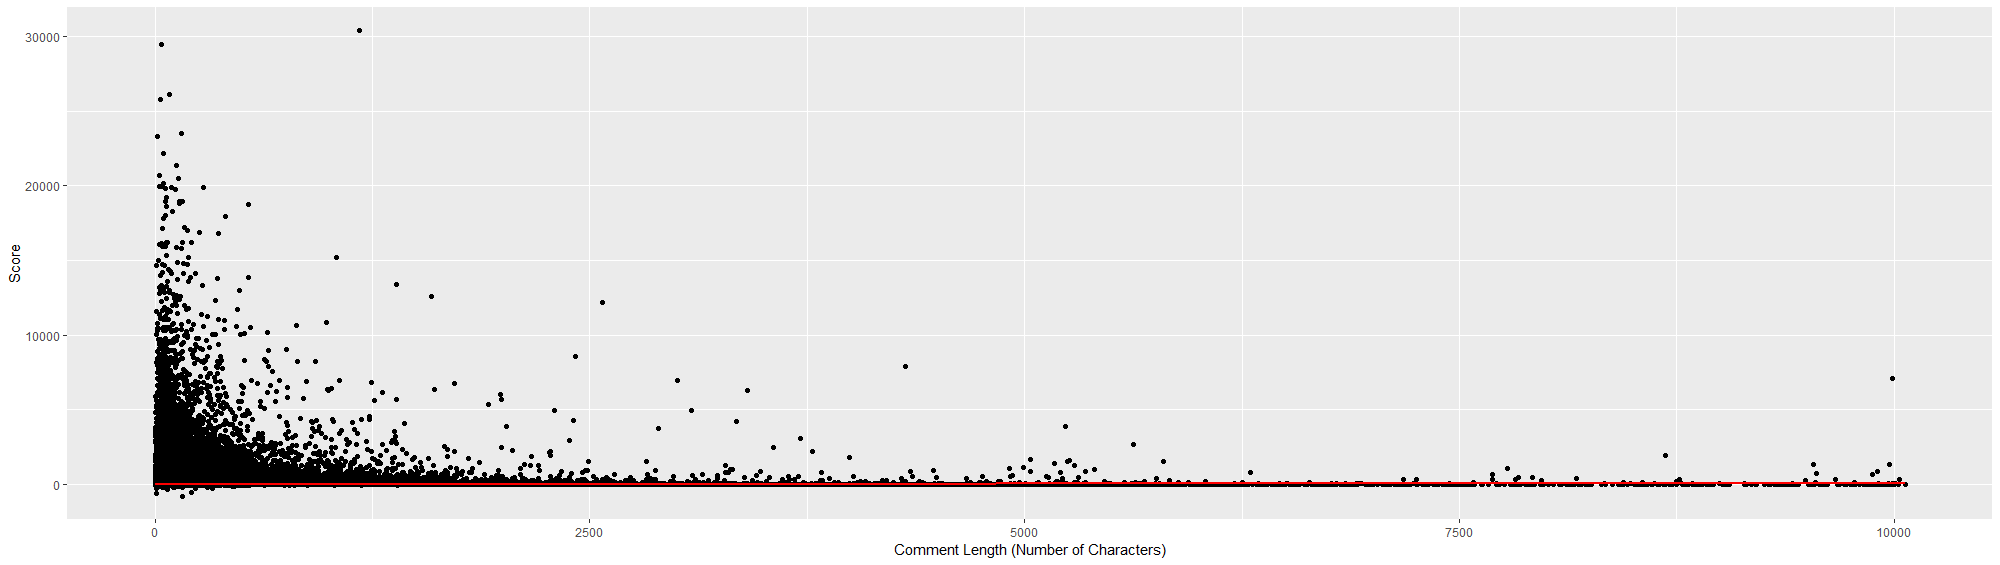
\includegraphics[width=1.0\textwidth]{graphs/length_score_all_subs}
        \caption{\textit{Length of comment versus the score}}
        \label{fig:scorevlen}
    \end{figure}
    
    A second attempt was made but this time the data was transformed to show the percent of successful comments at each particular length. The data was also grouped into 10 character chunks to help remove outliers. This new plot is shown in \autoref{fig:lenvscore} and \autoref{fig:lenvscore2} below.
    
    \begin{figure}[H]
        \centering
        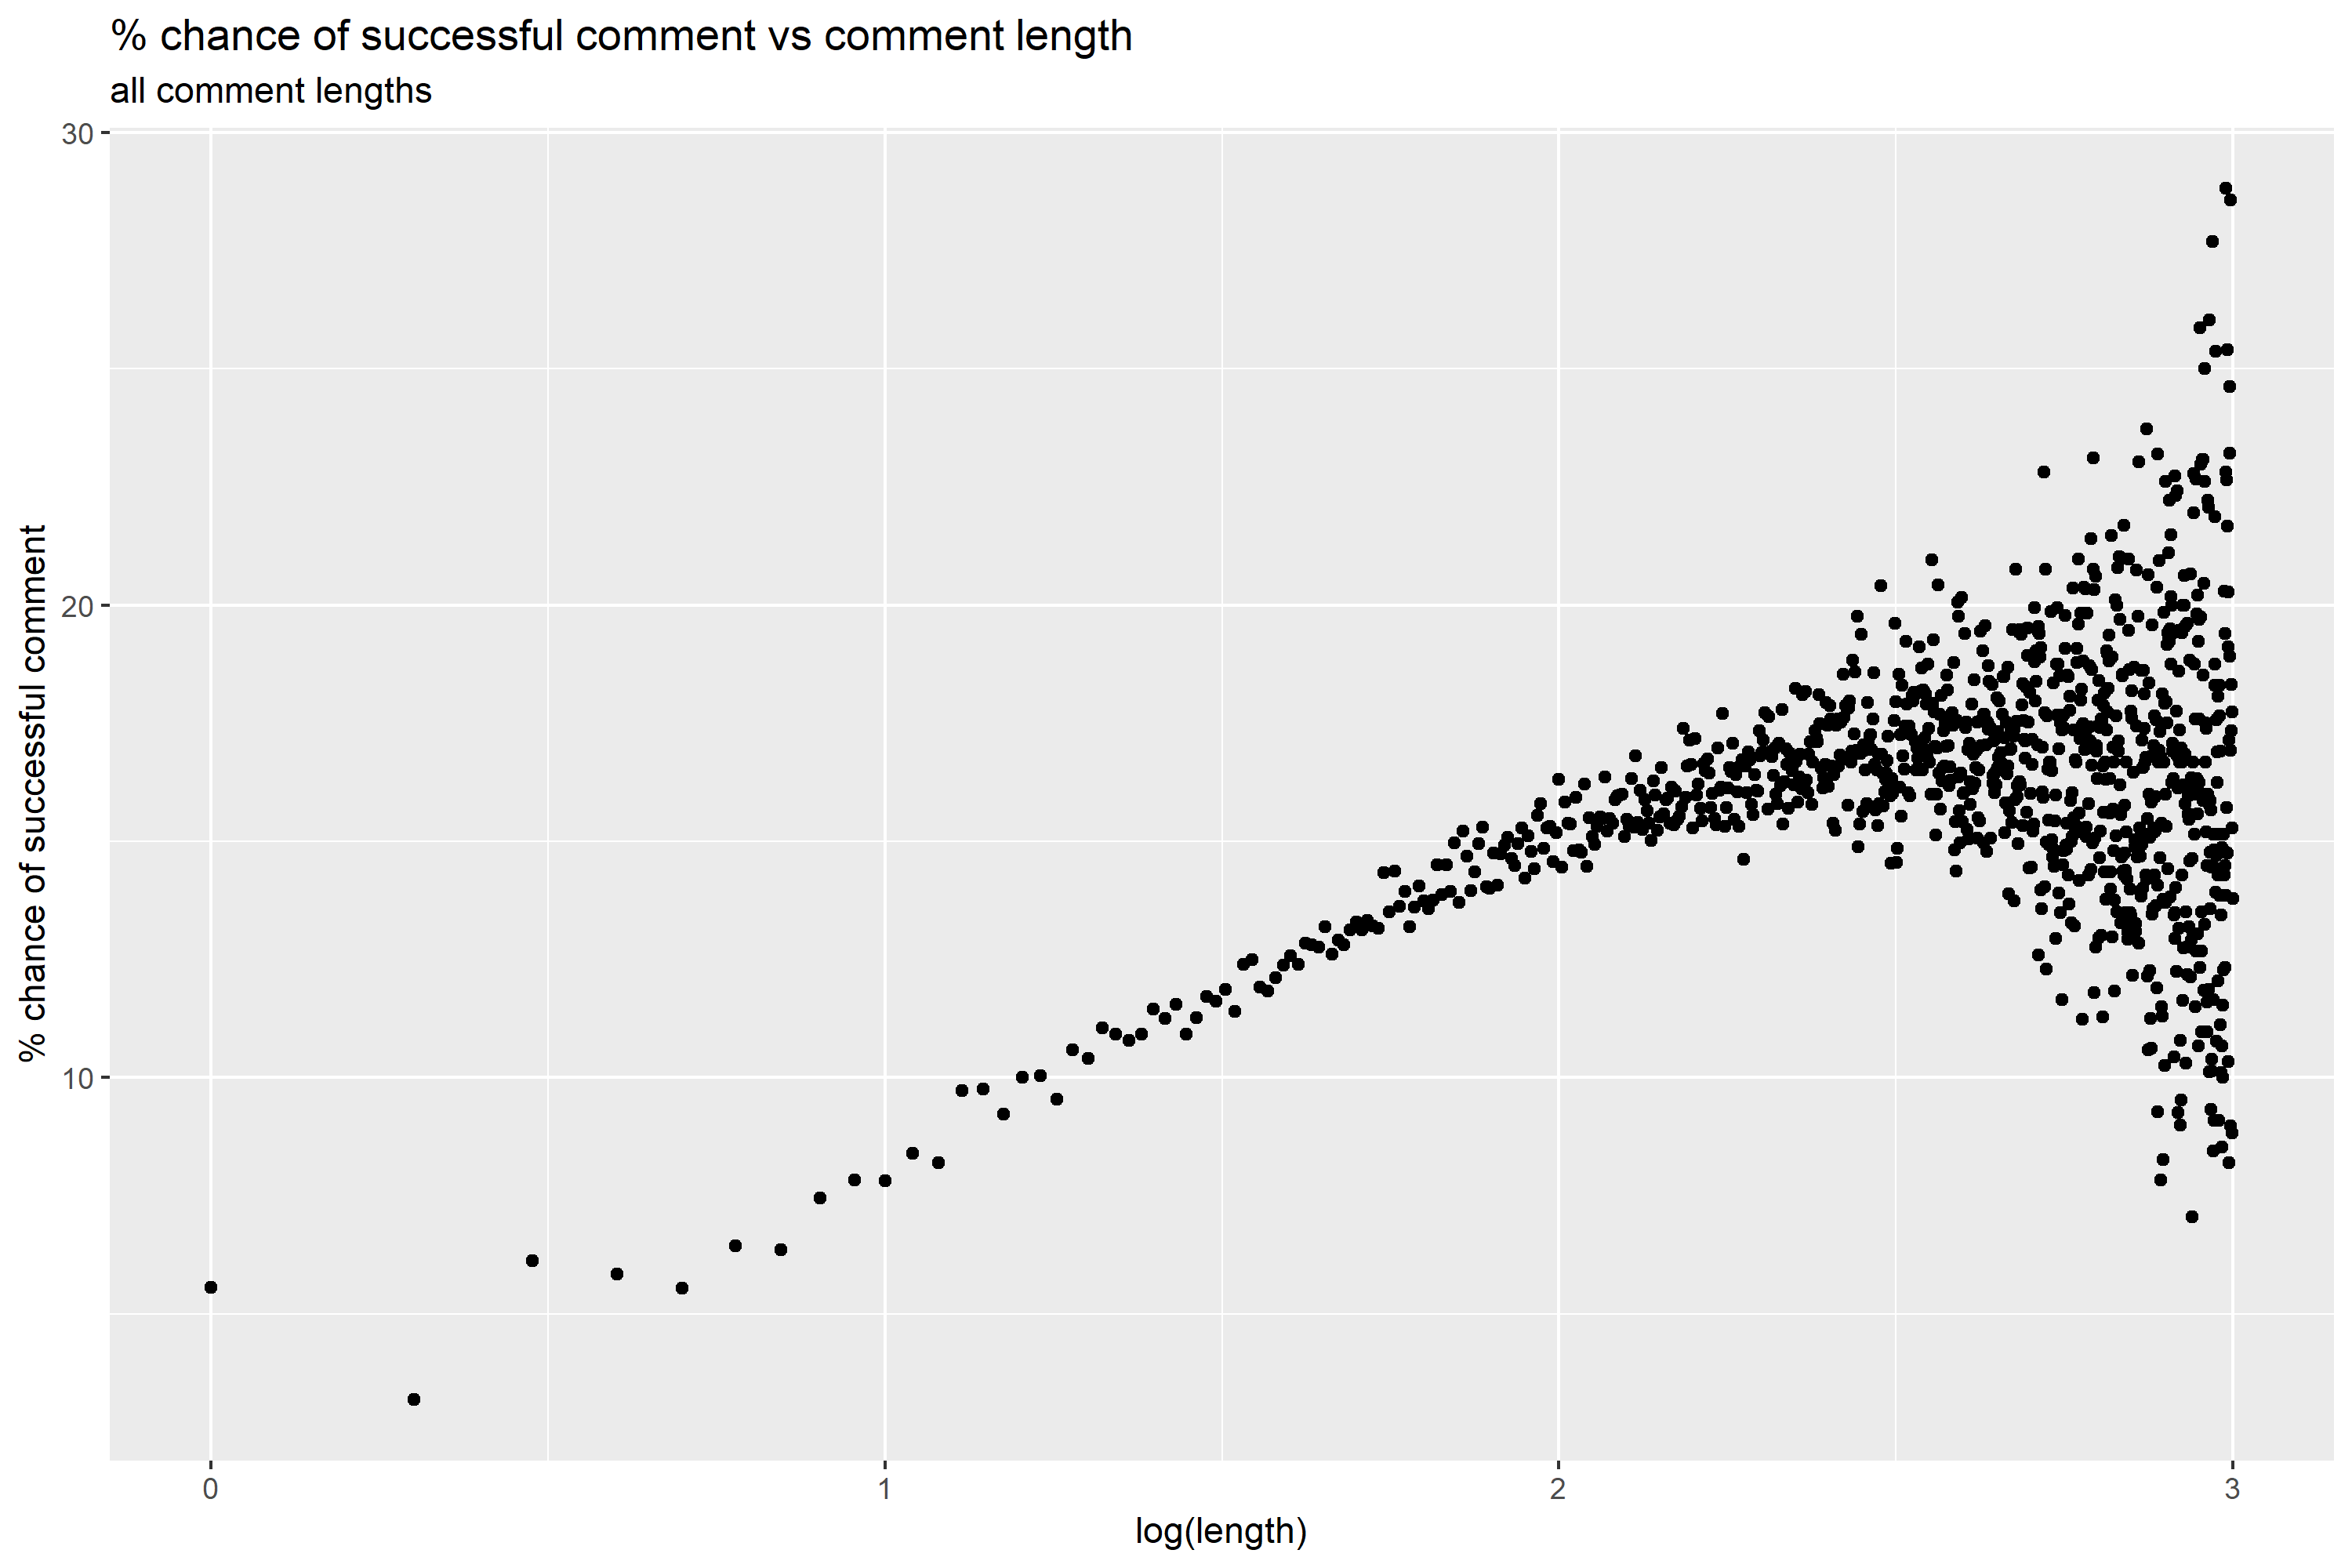
\includegraphics[width=1.0\textwidth]{graphs/lengthvsscore.png}
        \caption{\textit{Average score vs length where length is in 10 character chunks}}
        \label{fig:lenvscore}
    \end{figure}
    
    \begin{figure}[H]
        \centering
        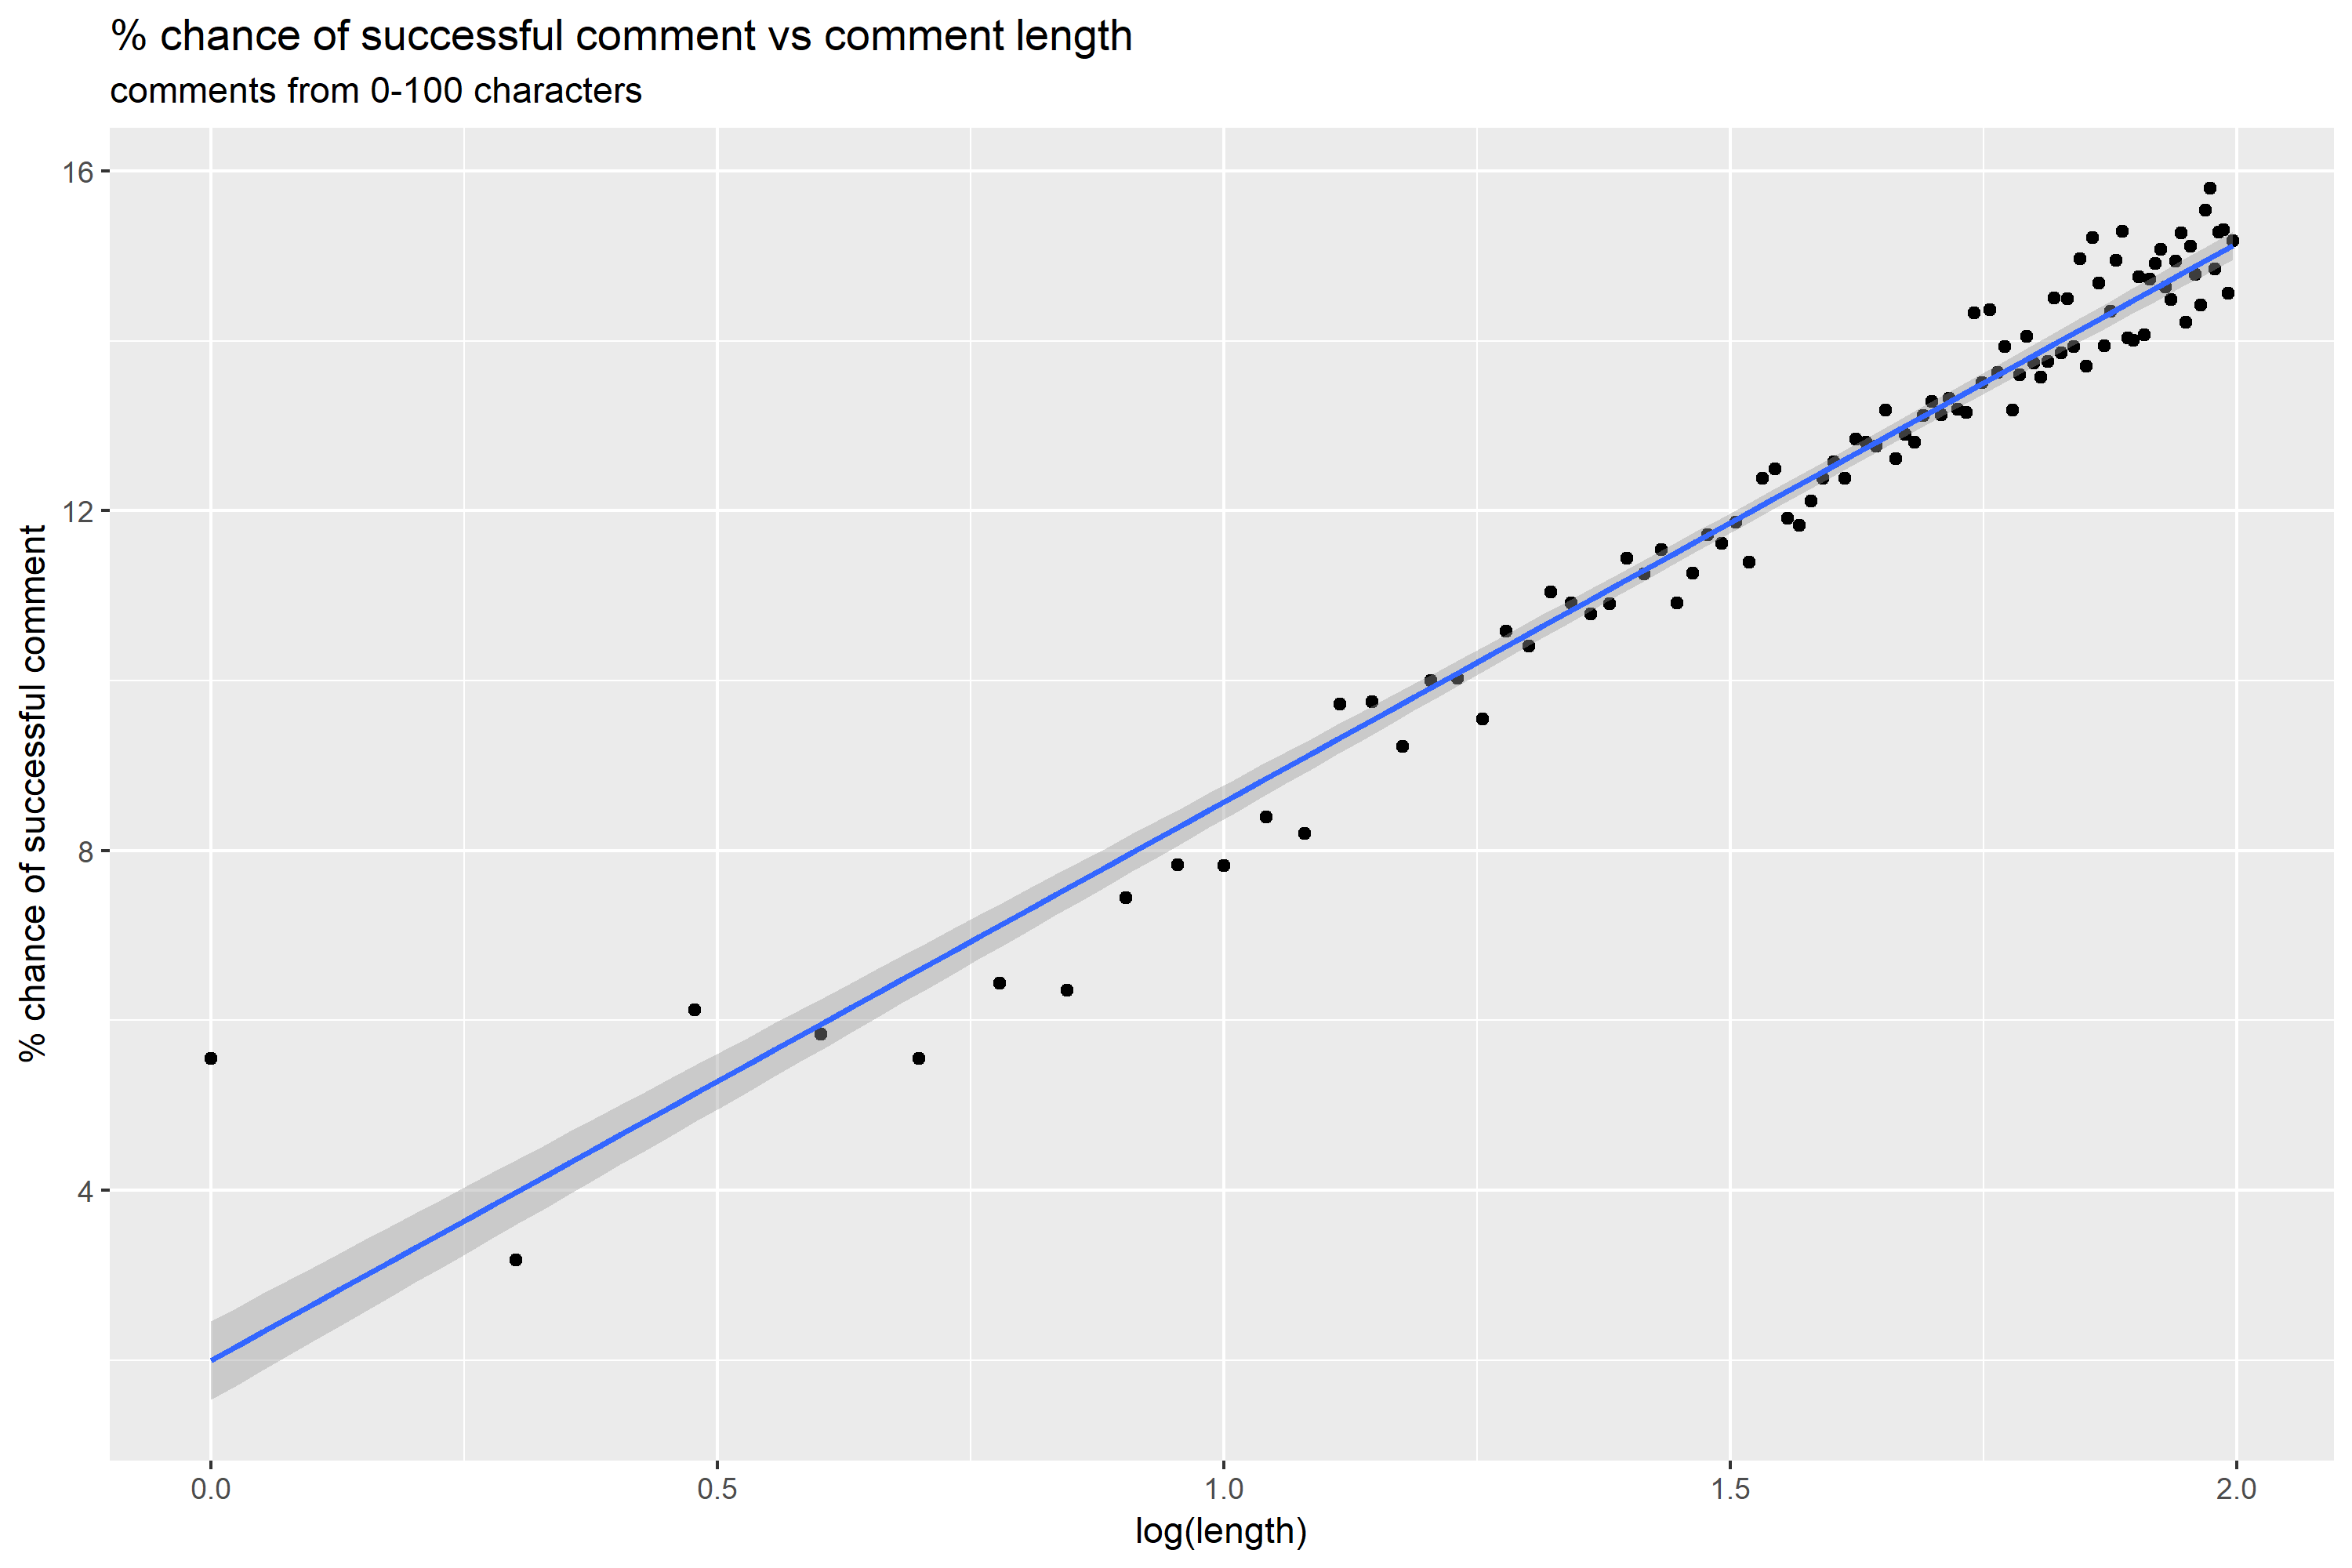
\includegraphics[width=1.0\textwidth]{graphs/lengthvsscore2.png}
        \caption{\textit{Same as \autoref{fig:lenvscore} but filtered to comments under 100 characters}}
        \label{fig:lenvscore2}
    \end{figure}

    Interestingly \autoref{fig:lenvscore} displays a linear relationship between length and score up to a length of around 100 characters, after which the score becomes unpredictable. It is believed that this is due to the lack of comments which exist at these lengths. \autoref{fig:lenvscore2} is the same plot but focused solely on the trend up to 100 characters, clearly indicating a linear relationship.
    
    The summary of this relationship is shown in \autoref{fig:lenvscoresum} below.
    
    \begin{figure}[H]
    \begin{lstlisting}
    Coefficients:
            Estimate Std. Error t value Pr(>|t|)    
(Intercept)  1.28544    0.18612   6.907 5.39e-10 ***
log(length)  3.04051    0.04947  61.462  < 2e-16 ***
---
Signif. codes:  0 ‘***’ 0.001 ‘**’ 0.01 ‘*’ 0.05 ‘.’ 0.1 ‘ ’ 1

Residual standard error: 0.4169 on 96 degrees of freedom
Multiple R-squared:  0.9752,	Adjusted R-squared:  0.975 
F-statistic:  3778 on 1 and 96 DF,  p-value: < 2.2e-16
    \end{lstlisting}
    \caption{\textit{Summary of the linear model from \autoref{fig:lenvscore2}}}
    \label{fig:lenvscoresum}
    \end{figure}
    
The code used to produce these graphs and summary can be found in \autoref{ch:Appendix} \autoref{sec:AppendexA6}


\subsection {Average Score vs Time Since Post}
    Another possible linear relation that was investigated was how much the average score of a comment varied based on the age of the post it was commenting on. Analysis showed that comments which were posted earlier were much more likely to get a higher score. The mean score quickly decreased as time progressed before flat-lining at around 100 5-minute intervals, which is approximately 8 hours. This is shown in \autoref{fig: timesincepost} below.
    
    \begin{figure}[ht]
        \centering
        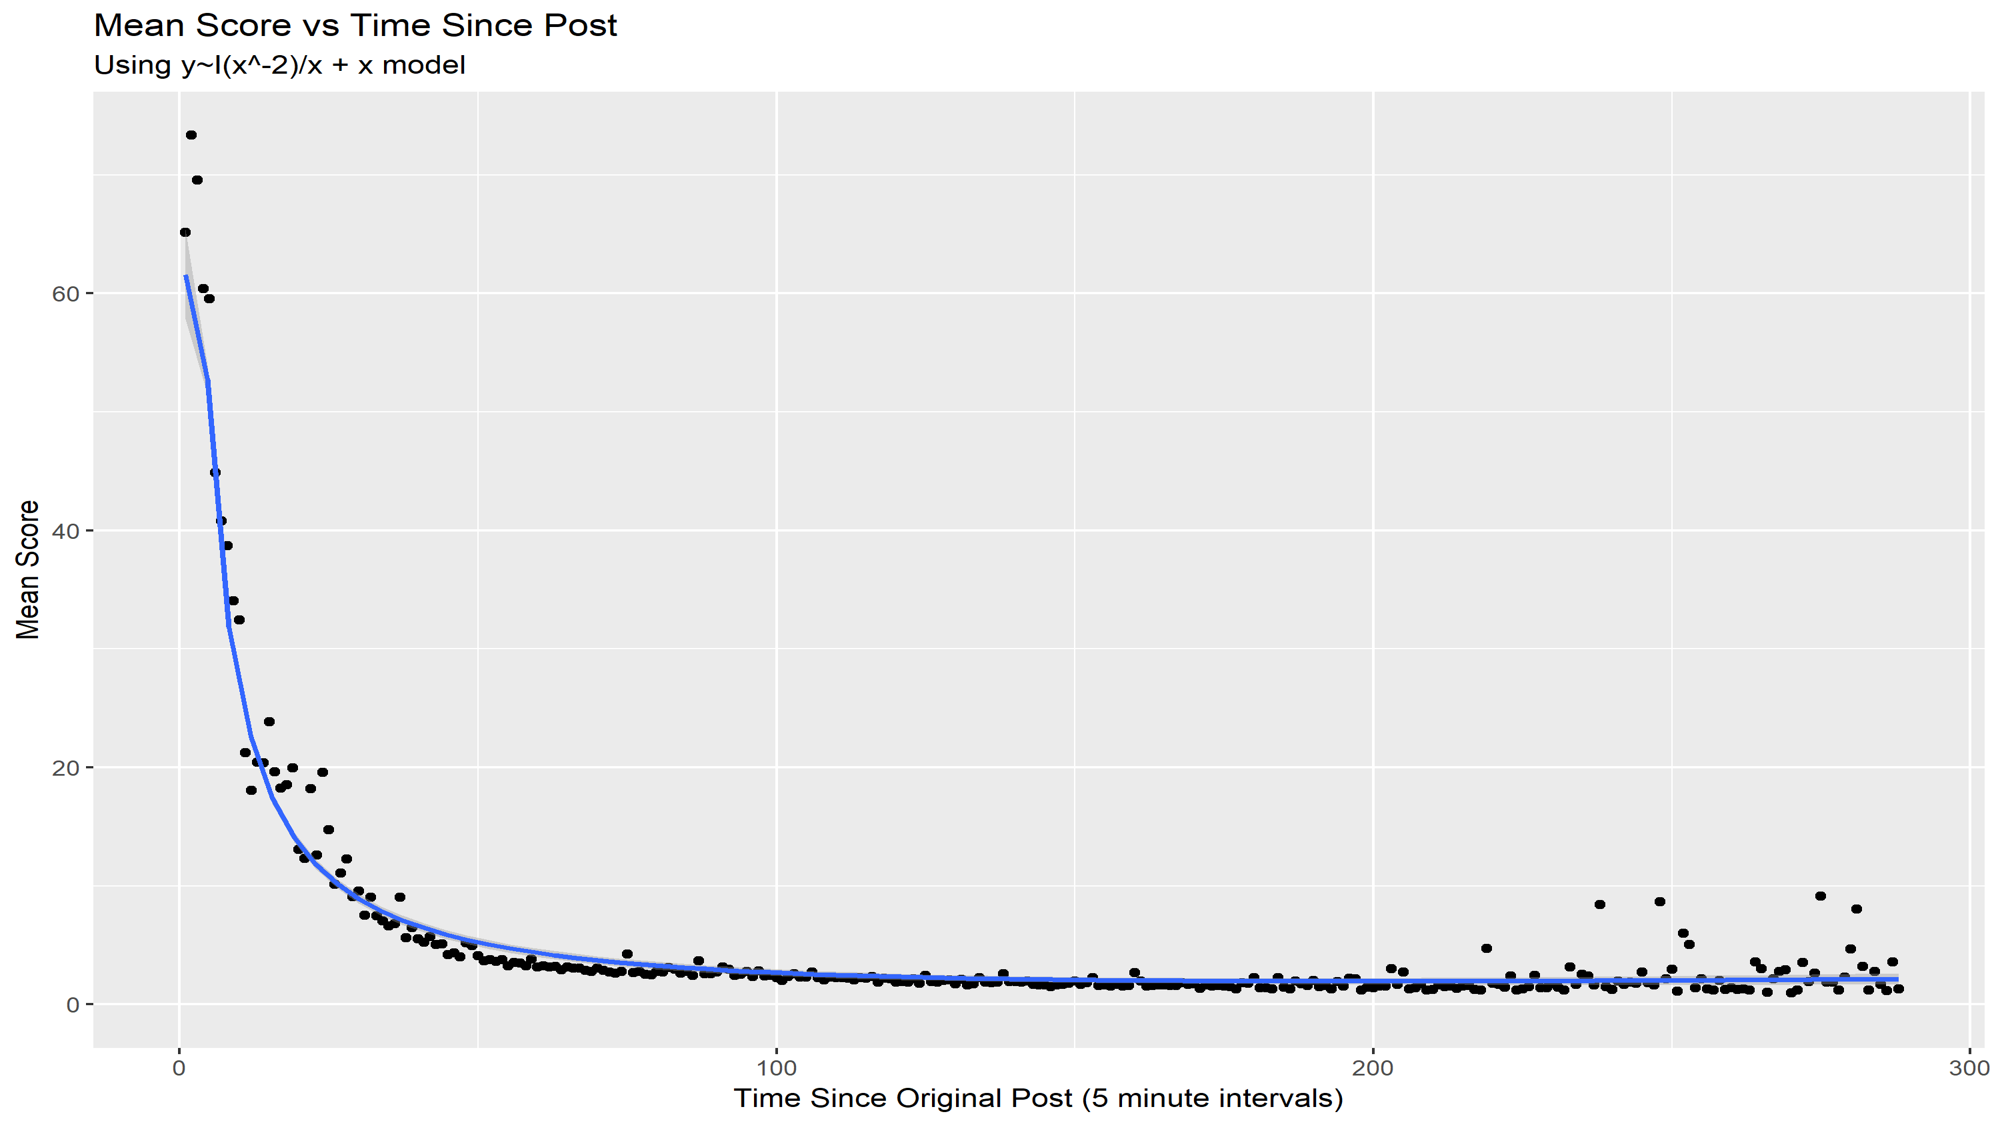
\includegraphics[width=1.0\textwidth]{graphs/meanscore_vs_time2}
        \caption{\textit{Mean Score versus time since post}}
        \label{fig: timesincepost}
    \end{figure}

It is clear from \autoref{fig: timesincepost} that the quicker a comment is created on a post, the more score it is expected to get. This conclusion is intuitive since earlier comments will be more visible to users visiting the comments section, and earlier comments will be seen by more users overall.

The summary of this relationship is shown in \autoref{fig:tspsum} below.

\begin{figure}[H]
    \begin{lstlisting}
Coefficients:
                Estimate Std. Error t value Pr(>|t|)    
(Intercept)      0.98419    0.09384   10.49   <2e-16 ***
I(dif^-2)     -217.18600    6.33142  -34.30   <2e-16 ***
I(dif^-2):dif  279.10738    5.21820   53.49   <2e-16 ***
---
Signif. codes:  0 ‘***’ 0.001 ‘**’ 0.01 ‘*’ 0.05 ‘.’ 0.1 ‘ ’ 1

Residual standard error: 2.752 on 953 degrees of freedom
Multiple R-squared:  0.8086,	Adjusted R-squared:  0.8082 
F-statistic:  2013 on 2 and 953 DF,  p-value: < 2.2e-16
    \end{lstlisting}
    \caption{\textit{Summary of the linear model from \autoref{fig: timesincepost}}}
    \label{fig:tspsum}
    \end{figure}

The code used to produce these graphs and summary can be found in \autoref{ch:Appendix} \autoref{sec:AppendexA7}

\subsection {Comment Tier vs Average Comment Score}
The next linear relation that was investigated was how the average score of a comment varies with how far down the comment chain that the comment was. The plot and linear model for this is shown in \autoref{fig: meanscorevscommenttier} below.

 \begin{figure}[H]
        \centering
        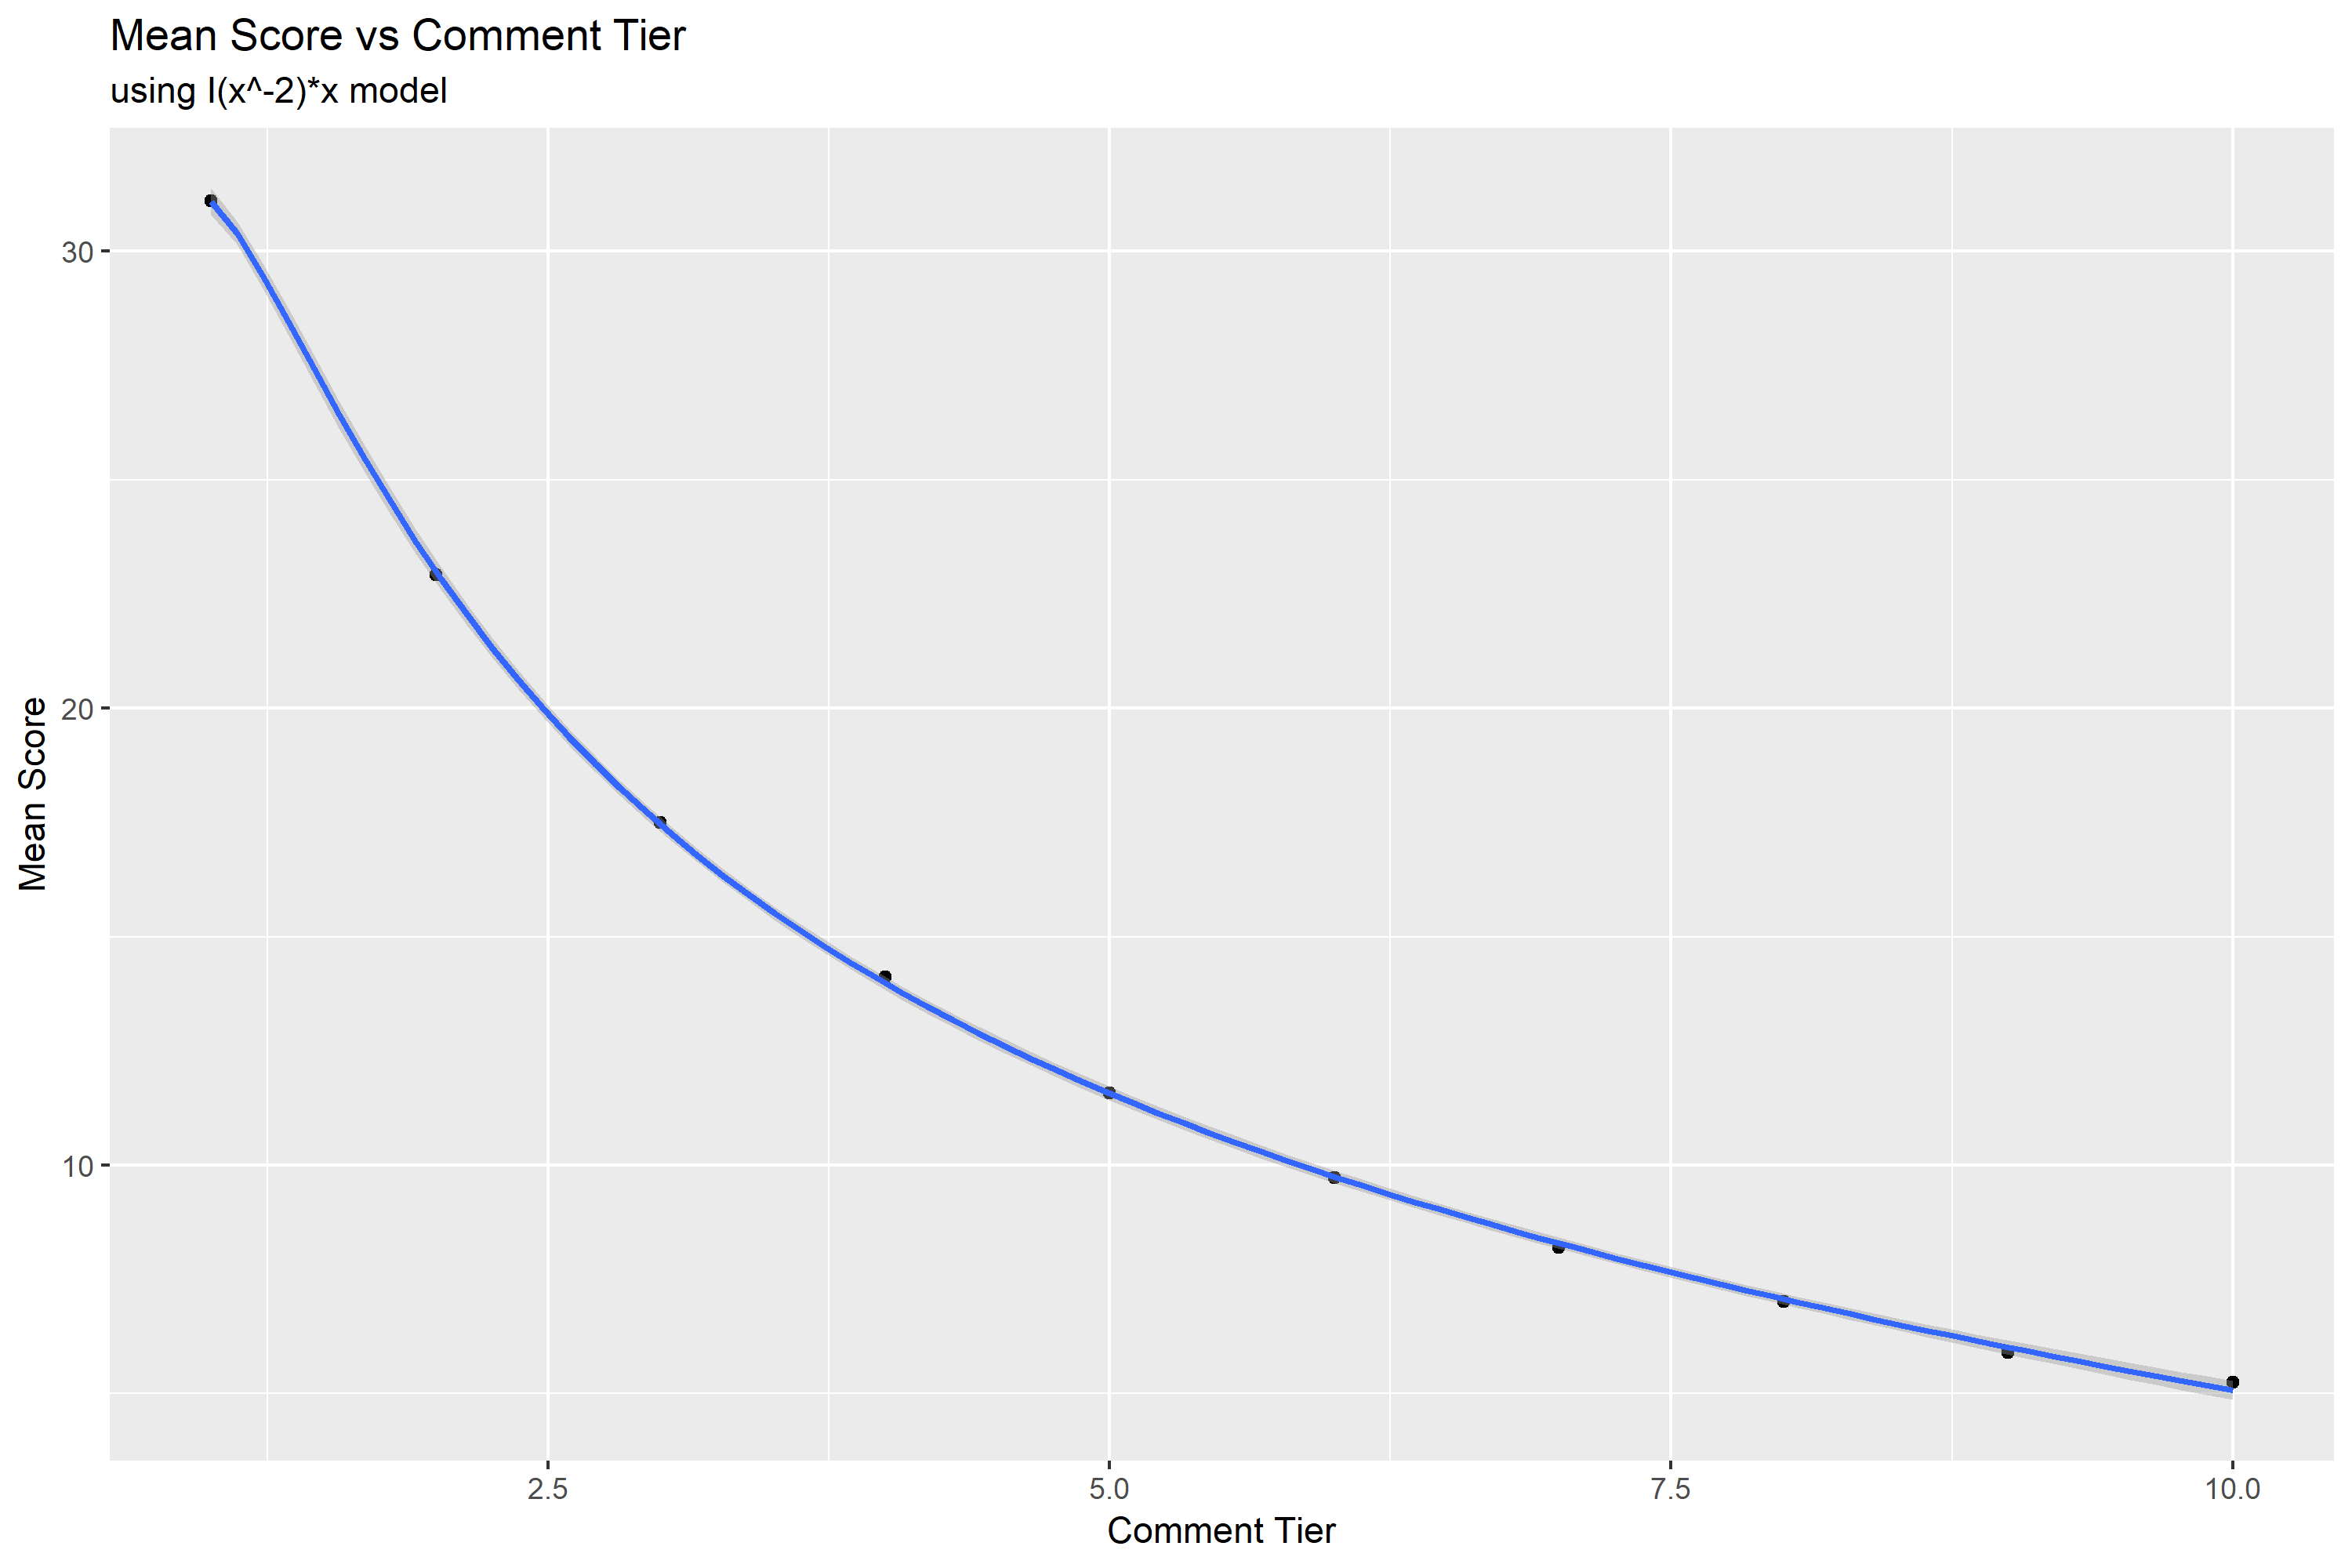
\includegraphics[width=1.0\textwidth]{graphs/meanscorevscommenttier.png}
        \caption{\textit{Mean Score vs Comment Tier}}
        \label{fig: meanscorevscommenttier}
    \end{figure}

As would be expected, the further down the comment tier a comment is, the less score it is expected to achieve. The summary of the linear model used is shown in \autoref{fig:commenttiersum} below, and the code used to produce the plot can be found in \autoref{ch:Appendix} \autoref{sec:AppendexA8}.

\begin{figure}[H]
    \begin{lstlisting}
Coefficients:
                 Estimate Std. Error t value Pr(>|t|)    
(Intercept)       4.75229    0.55055   8.632 0.000133 ***
I(tier^-2)      -22.97098    1.19209 -19.269 1.26e-06 ***
tier             -0.44247    0.04607  -9.604 7.29e-05 ***
I(tier^-2):tier  49.74669    1.65659  30.030 9.05e-08 ***
---
Signif. codes:  0 ‘***’ 0.001 ‘**’ 0.01 ‘*’ 0.05 ‘.’ 0.1 ‘ ’ 1

Residual standard error: 0.1169 on 6 degrees of freedom
Multiple R-squared:  0.9999,	Adjusted R-squared:  0.9998 
F-statistic: 1.533e+04 on 3 and 6 DF,  p-value: 4.853e-12
    \end{lstlisting}
    \caption{\textit{Summary of the linear model from \autoref{fig: timesincepost}}}
    \label{fig:commenttiersum}
    \end{figure}
    
\subsection{Average Score vs Time of Day}
How the average score of a comment varied based on the time of day was also found for all days of the week. Even though no linear modelling was carried out on this specific data, it would still be extremely important information to know in order to try to maximise the score that a comment received. \autoref{fig: avgscorevstimeofday} below shows how the average score varied over the course of a day, for all days of the week.

 \begin{figure}[H]
        \centering
        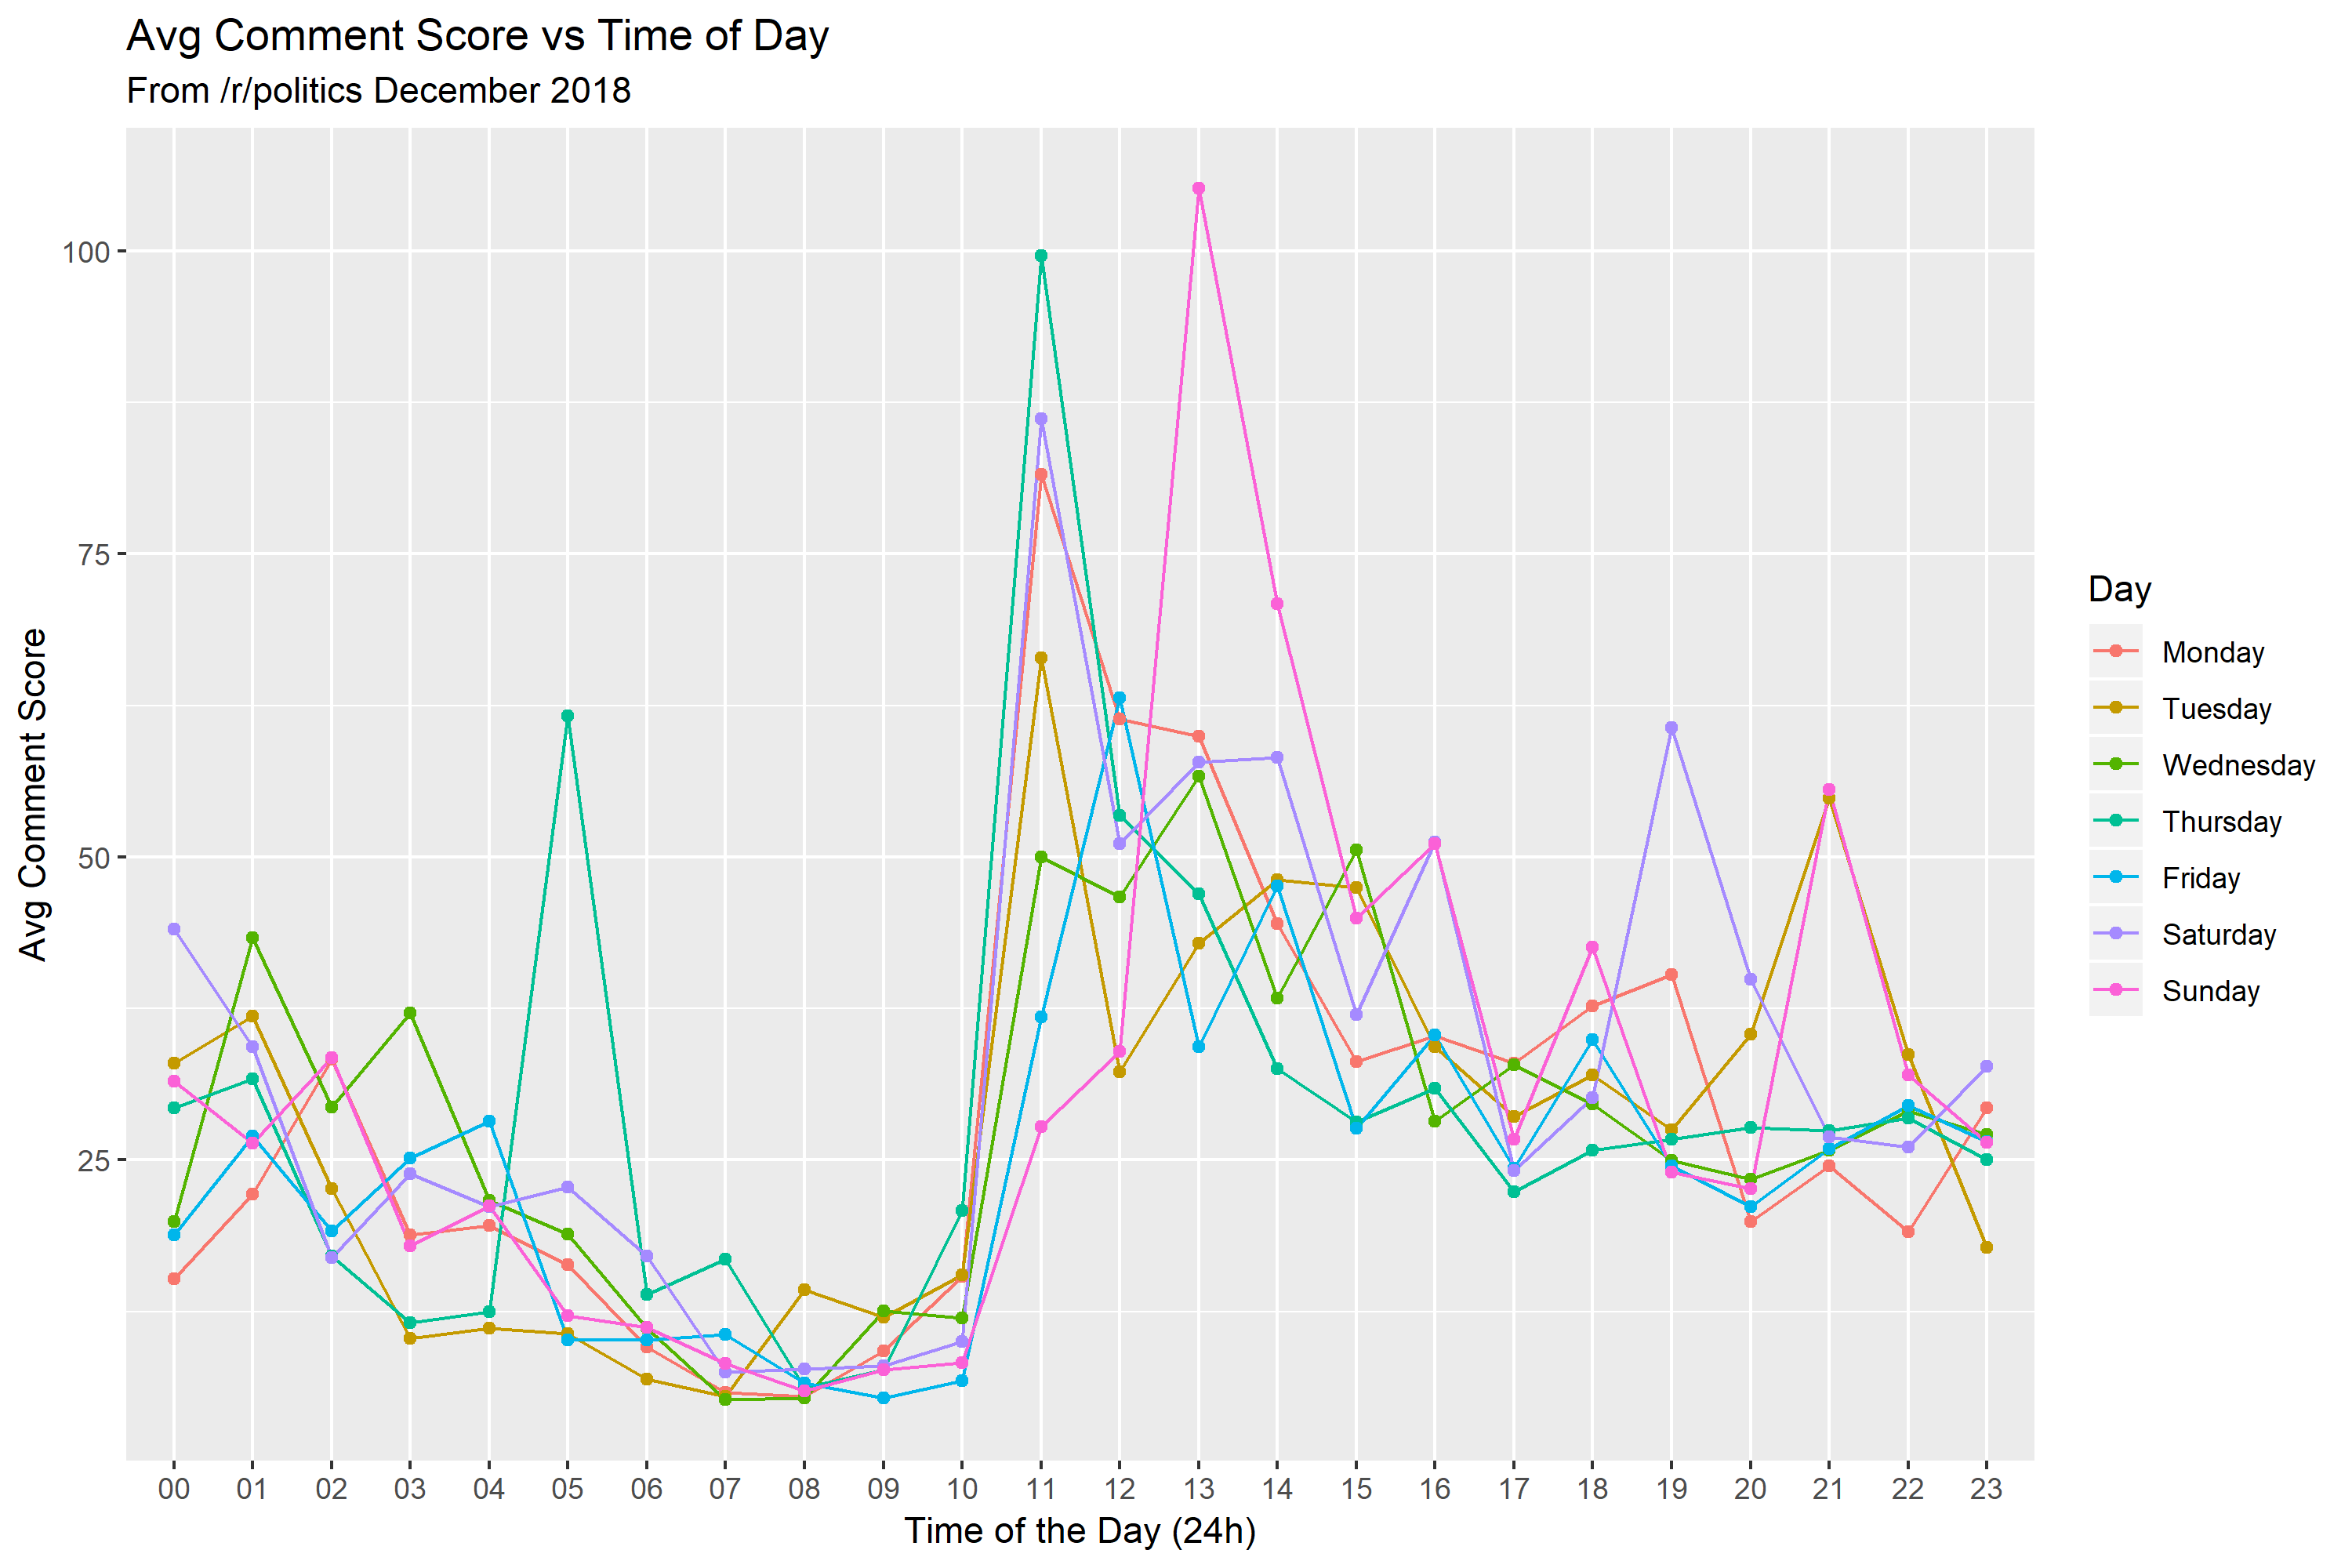
\includegraphics[width=1.0\textwidth]{graphs/avgscorevstimeofday.png}
        \caption{\textit{Average score over the course of the day for all days of the week}}
        \label{fig: avgscorevstimeofday}
    \end{figure}
    
As can be seen the average score is its highest around 12pm, and lowest around 9am, with weekends achieving overall higher scores. Thus to achieve the greatest chance of a high comment score, posting the comment midday at the weekend would give the highest chance of success. The code which generate the above plot can be found in \autoref{ch:Appendix} \autoref{sec:AppendexA9}

\section{Classification using a Neural Network}
\label{sec:NNclass}
Through attempts to generate a predictive model of score, it became clear the the words used within a comment were likely to be extremely important. However, it was not immediately clear how to best approach using text-analysis as a predictor. Simple models were initially made comparing the use of popular community words against score and no correlation was found. It was therefore decided to adopt a machine learning approach using the \textit{Keras} package as outlined in \autoref{sec:neuralnet}

The first neural network created simply took as input the words used within the body of a comment. These words were converted into a matrix as described in \autoref{sec:neuralnet} and used as an input for the neural network. Note, for this experiment, in an attempt to reduce the variables involved, only tier 1 comments were used. Due to this, the average score, which is an indicator of a comments success, had increased to 31 points. The training history of the first neural network attempt is shown in \autoref{fig:neural1} below.

 \begin{figure}[H]
        \centering
        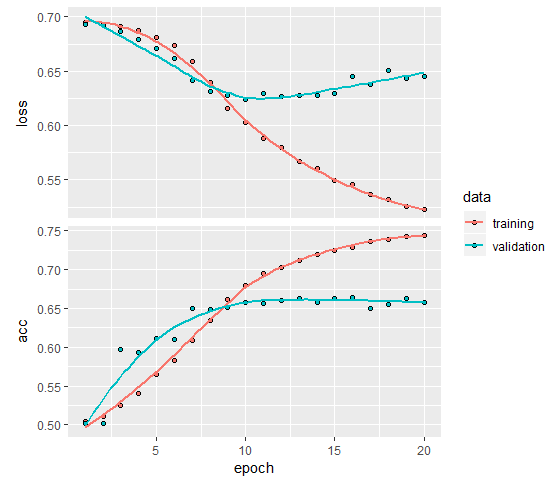
\includegraphics[width=1.0\textwidth]{graphs/neural1.png}
        \caption{\textit{History of a neural network of comment content. acc = accuracy}}
        \label{fig:neural1}
    \end{figure}

The neural network achieved a training accuracy of around 75\%, and a validation accuracy of around 66\%. This difference is due to the over-fitting of the data that occurs around epoch 9. Using the model as a predictor on a set of testing data revealed a classification accuracy of 67\%.

From an analysis of the data it was noticed that the topic of the post which the comment is in would be a powerful predictor of score. More popular post topics would attract more users, and thus comments within the post would achieve a higher average score. The above process of creating a neural network was repeated except the name of the post was extracted from the permalink field of the data. The words contained within the post name were then combined with the body and fed into the neural network again. The result of the training process is shown in \autoref{fig:neural2} below.

 \begin{figure}[H]
        \centering
        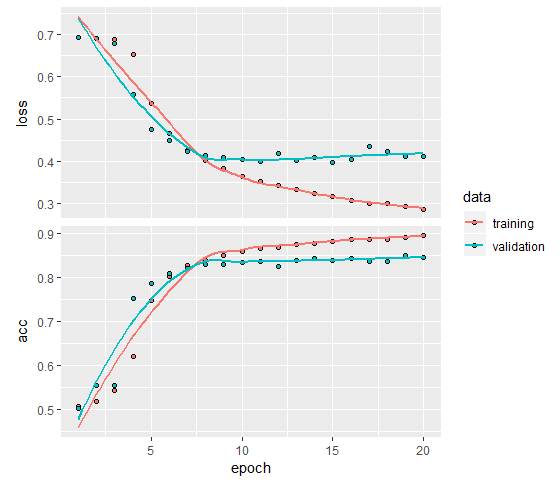
\includegraphics[width=1.0\textwidth]{graphs/neural4.png}
        \caption{\textit{History of the second neural network of comment content and post name}}
        \label{fig:neural2}
    \end{figure}

This new neural network achieved a training accuracy of 89\% and a validation accuracy of 85\%. Much like the first attempt it also experienced overfitting around epoch 9. When used on the same set of testing data as before, it achieved a classification accuracy of 84\%.

The code used to create this neural network is shown in \autoref{ch:Appendix} \autoref{sec:AppendexNeural}


